% 第2章 キャッシュフローと時間価値(資料2)
\chapter{キャッシュフローと時間価値}

本章から数理的な議論に入る。鍵となる概念は「お金の価値は受け取る時点によって
異なる」という\textbf{時間価値} (time value) の考え方である。将来のキャッシュ
フローが確定的な場合に，ある時点のキャッシュフローを(経済学的に等価な)異なる
時点のキャッシュフローに変換する方法---現在から将来へ，将来から現在へ---を学び，
その応用として投資の価値評価法(NPV法・IRR法)を扱う。題材としては，キャッシュ
フローが単純で有価証券の代表例である債券を用いる。

\section{債券}

\subsection{債券のキーワード}

債券の特性を示すキーワードとして，以下を押さえておく。

\begin{itemize}
\item \textbf{額面} (face value)：償還時に返済される金額。
\item \textbf{満期} (maturity)：元本が償還される時点。
\item \textbf{券面利率}(クーポンレート，coupon rate)：利息計算に使われる利率。
これに基づいて支払われる利札を\textbf{クーポン} (coupon) という。
\item \textbf{利払頻度}：年払い，半年払いなど。
\item \textbf{発行体} (issuer)：債券を発行して資金を調達する主体。
\item \textbf{信用格付け} (credit rating)：発行体の信用力の評価。
\end{itemize}

\subsection{キャッシュフローによる分類}

\begin{description}
\item[利付債] 満期まで定期的に利払が行われる債券。満期に額面分が償還されることを
\textbf{満期一括償還}という。満期一括償還債では，満期に利払額と償還額の合計額が
支払われる。
\item[割引債] 利払がなく，満期に額面分の金額が償還される債券。
\end{description}
なお，上記に該当しない，元本を分割して償還するアモチ型の債券もある。

その他の分類として，
\begin{itemize}
\item \textbf{有期債}(満期のあるもの)と\textbf{永久債}(満期のないもの)，
\item \textbf{固定利付債}(券面利率が一定)と\textbf{変動利付債}(券面利率が変動する)，
\end{itemize}
がある。

\subsection{発行体による分類}

\begin{description}
\item[国債] 国が発行している債券。発行額も発行頻度も高く，知名度は債券で
No.~1。多くは金融機関や機関投資家向けだが，個人向けの国債もある。
\item[政府保証債] 政府関係機関や特殊法人が発行する債券で，政府による支払保証が
ついているもの。
\item[地方債] 地方公共団体が発行している債券。
\item[社債] 一般事業会社が発行している債券。いろいろな種類と条件のものがある。
\item[電力債] 各地方の電力会社が発行している債券。発行額が大きい。
\end{description}

\subsection{キャッシュフローの図示}

キャッシュフロー(以下 CF と略すことがある)の作図には次の約束を設ける。
時刻を横軸にとり，キャッシュフローは発生時刻上の縦方向の矢印で示す。
\textbf{正(受取)は上向き，負(支払)は下向き}である。縦のスケールを正確に
書くとわかりにくい場合は，適当に歪めて書いてよい。

\subsection{固定利付債のキャッシュフロー}

固定利付債のキャッシュフローを定式化する。
\begin{itemize}
\item 利払日：$t_i$ ($i=1,2,\dots,m$;\ $t_m$：満期，$t_0=0$)。時刻は年単位で表す。
\item 額面：$F$。
\item クーポンレート：$K$(\emph{必ず年率で表示})。
\item クーポン：
\begin{equation}
C_i = K \times F \times (t_i - t_{i-1}).
\label{eq:coupon}
\end{equation}
\end{itemize}
式\eqref{eq:coupon}は，「年率 $K$ の利息が，期間 $(t_i-t_{i-1})$ 年分だけ額面 $F$ に
対して付く」ことを表している。期間 $(t_i - t_{i-1})$ も年単位で表示することに注意。

\begin{figure}[htbp]
\centering
\begin{tikzpicture}[scale=1.1]
\draw[-{Stealth}] (0,0) -- (9.5,0) node[right]{$t$};
\fill (0,0) circle (1.5pt) node[below=1mm]{$0$};
\foreach \x/\lab in {1.5/t_1, 3/t_2, 5.5/t_i, 7.5/t_m}{
  \node[below] at (\x,-0.05) {$\lab$};}
\draw[-{Stealth}, thick] (1.5,0) -- (1.5,0.8) node[above]{$C_1$};
\draw[-{Stealth}, thick] (3,0) -- (3,0.8) node[above]{$C_2$};
\node at (4.2,0.5) {$\cdots$};
\draw[-{Stealth}, thick] (5.5,0) -- (5.5,0.8) node[above]{$C_i$};
\node at (6.5,0.5) {$\cdots$};
\draw[-{Stealth}, thick] (7.4,0) -- (7.4,0.8) node[above]{$C_m$};
\draw[-{Stealth}, very thick] (7.6,0) -- (7.6,2.0) node[above]{$F$};
\end{tikzpicture}
\caption{固定利付債のキャッシュフロー。満期 $t_m$ にはクーポン $C_m$ に加えて
額面 $F$ が償還される。}
\label{fig:fixedbond-cf}
\end{figure}

\begin{example}[固定利付債のキャッシュフロー]
満期2年，年2回払，クーポンレート4\%，額面100円の固定利付債を考える。
利払日は $t_i = i/2$ 年($i=1,2,3,4$;満期2年)であり，クーポンは
式\eqref{eq:coupon}より
\[
C_i = 4\% \times 100 \times 0.5 = 2 \text{ 円}
\]
となる。すなわち，0.5年後，1年後，1.5年後に2円ずつ，2年後にクーポン2円と
額面100円の合計102円を受け取る。
\end{example}

\begin{example}[割引債のキャッシュフロー]
満期2年，額面100円の割引債を考える。利払はなく，キャッシュフローは満期日
(2年後)の100円のみである。
\end{example}

\vspace{18pt}

\subsection{変動利付債のキャッシュフロー}

変動利付債では，クーポンレートが市場金利に連動して変動する。従来の標準物では
クーポンレートとして 6M-LIBOR(6ヶ月物LIBOR金利)$L_{i-1}$ が使われ，クーポンは
\begin{equation}
C_i = F \, L_{i-1} (t_i - t_{i-1})
\end{equation}
で与えられた。ここで重要なのは添字が $i-1$ であることである。すなわち，標準物では
クーポンレートは\emph{前回の利払日} $t_{i-1}$ に決まり，利払日 $t_i$ の利息額は
前回の利払日 $t_{i-1}$ の時点で確定する。これは「借りる時に利子は既知」という
原則に沿ったものである。

\begin{remark}[LIBORの廃止と後決め金利]
2021年末，LIBORは代表的な変動金利ではなくなった。現在の変動利付債では，日々の
「当日から翌日までの金利」(オーバーナイト金利，ON金利)による複利運用の
一定期間分の成果をまとめて払う方式が使われている。

例として，今から半年後の利息額を考える。$t$ 日目のオーバーナイト金利 $r_t$ は
その当日に確定する。$t$ 日目の1円は，$t+1$ 日には $1 + r_t \Delta t$ 円になる
($\Delta t$:1日の年換算値)。これを半年分積み重ねる(=掛け続ける)と，
半年後には
\[
(1 + r_0 \Delta t)(1 + r_1 \Delta t) \cdots (1 + r_{\text{半年後}-1} \Delta t)
\]
となり，半年前の1円との差(=半年間で増えた分)
\[
(1 + r_0 \Delta t)(1 + r_1 \Delta t) \cdots (1 + r_{\text{半年後}-1} \Delta t) - 1
\]
が利息額になる。この利息額が確定するのは，$t=0$ ではなく
$t = \text{半年後} - \Delta t$ の時点である。

このように，従来の変動金利は\textbf{先決め金利}(今回の利払日の利息額は前回の
利払日に確定)であったのに対し，現在の変動金利は\textbf{後決め金利}(今回の
利払日の利息額は今回の利払日の直前に確定)である。これによって，金利デリバティブに
よっては評価方法が変更されたものもある。
\end{remark}

\vspace{18pt}

\section{時間，価値，利回り}

本節では，将来が確定的な場合を考え，ある時点の CF を(経済学的に等価な)異なる
時点の CF に変換する方法を学ぶ。

\subsection{現在価値の考え方}

将来のキャッシュフローが確定している場合を考える(確定的でない場合を扱うのが，
本講義後半のデリバティブの価格付け理論である)。

1円投資したとき，1年後に $(1+R)$ 円が確実に返ってくる場合を考える。1円は元本，
$R$ 円は利息(利子)である。このとき，\textbf{1年後の1円の現在価値(現時点に
おける価値)} $D(1)$ はいくらだろうか(記号 $D(1)$ の $1$ は「1年後」の意味)。

これは比例計算で算出できる：
\[
\begin{array}{ccc}
1 \text{ 円} & \longrightarrow & 1+R \text{ 円}\\
D(1) \text{ 円} & \longrightarrow & 1 \text{ 円}
\end{array}
\qquad\Longrightarrow\qquad
D(1) = \frac{1}{1+R}.
\]
左側の金額を\textbf{現価(現在価値)}，右側の金額を\textbf{終価}と呼ぶ。

\subsection{利回り}

\begin{definition}[利回り]
\textbf{利回り}とは，単位時間あたりの平均利子率である。利回りは年率(単位時間は
1年)で表示するのが原則である。
\end{definition}

利回りにはいろいろな考え方があり，一番大きなポイントは\textbf{利息を再投資するか
否か}である。また，年あたりの再投資回数を\textbf{転化回数}という。

\subsection{再投資と現在価値}

前述の例は1年を1期間として考えたケースであった。では，半年ごとに再投資が可能
(転化回数 $m=2$)だとしたらどうなるか。半年を1期間とみなせば，1年間は2期間に
なる。ここで注意すべきは，\emph{利率 $R$ は年率で定義されている}という約束事で
ある。$m=2$ のときの1期間は半年であり，その間に増えるのは比率 $R/2$ である。
したがって比例計算により
\[
\begin{array}{ccccc}
1 \text{ 円} & \to & 1+R/2 \text{ 円} & \to & (1+R/2)^2 \text{ 円}\\
D(1) \text{ 円} & \to & & \to & 1 \text{ 円}
\end{array}
\qquad\Longrightarrow\qquad
D(1) = \frac{1}{(1+R/2)^2}.
\]
一般に，転化回数 $m$(=$1/m$ 年ごとに再投資が可能)ならば，
\begin{equation}
1 \text{ 円} \to \cdots \to \Bigl(1+\frac{R}{m}\Bigr)^m \text{ 円},
\qquad
D(1) = \frac{1}{(1+R/m)^m}.
\label{eq:D1m}
\end{equation}

\subsection{利息を再投資しない場合とする場合}

\paragraph{利息を再投資しない場合。}
利息をその後の投資にまわさず，回収する場合を考える。1回の投資期間が半年
($1/2$年)ならば，1年で投資を2回繰り返す。年間の利息は，1回の投資期間(半年)で
得られる利息の2倍になる(ただし，1回の投資期間で得られる利息は年率の $1/2$)。
すなわち，元本1円に対して1年で得られる利息は
\[
\frac{R}{2} \times 2 = R \text{ 円}.
\]
同様に，1回の投資期間が3ヶ月($1/4$年)ならば1年で投資を4回繰り返し，年間の
利息は $\frac{R}{4}\times 4 = R$ 円となる。つまり，再投資しなければ，転化回数に
よらず年間の利息は $R$ 円である。

\paragraph{利息を再投資する場合。}
利息全額をその後の投資にまわす場合を考える。1回の投資期間が半年ならば，1年後の
総価値は1回の投資(半年)で得られる価値の2乗となる：
\[
1 \text{ 円} \to 1 + \frac{R}{2} \text{ 円} \to \Bigl(1+\frac{R}{2}\Bigr)^2 \text{ 円}.
\]
1年で得られる利息は $(1+R/2)^2 - 1$ 円である。1回の投資期間が3ヶ月ならば，
1年後の総価値は $(1+R/4)^4$ 円になる。

\subsection{単利と複利}

利回りには，\textbf{単利}と\textbf{複利}がある。

\begin{description}
\item[単利] 利子を再投資\emph{しない}で得られる利回り。一般に，単利の利回りは
\[
\text{(単利利回り)} = \frac{\text{(受取金額)}-\text{(支払金額)}}
{\text{(支払金額)}\times\text{(期間)}}
\]
という形，すなわち「単位時間で，どのくらいの比率だけ増えたか」で計算される。
額面 $F$，クーポンレート $K$(年 $m$ 回払い)，満期 $T$ 年後の債券が，現在
$p$ 円で取引されているとすると，利回り(単利)は
\begin{equation}
\frac{\dfrac{1}{p}\Bigl(F + F \times \dfrac{K}{m}\times m \times T - p\Bigr)}{T}
= \frac{F-p}{pT} + \frac{FK}{p}
\end{equation}
となる。特に $K=0$(割引債)ならば $\dfrac{F-p}{pT}$，$F=p$(パー)ならば $K$ と
なる。なお，この単利利回りが，そのまま(複利の)利回り $R$ になるわけではない
ことに注意する。
\item[複利] 利子を全額再投資して得られる利回り。再投資の間隔により，1年複利，
半年複利，3ヶ月複利，…がある。投資の一期間の長さによって，同じ利回りでも終価は
異なる。
\end{description}

\subsection{複利による終価と現価}

複利の場合の1年後の関係を整理する。利子率を年率 $R$ とすると，
\begin{itemize}
\item 半年ごとに再投資($m=2$):$1$ 円 $\to (1+R/2)^2$ 円，
$D(1) = (1+R/2)^{-2}$。
\item $1/m$ 年ごとに再投資：$1$ 円 $\to (1+R/m)^m$ 円，
$D(1) = (1+R/m)^{-m}$。
\end{itemize}

\begin{example}[複利による終価]
利子率(年率)を10\%とする。1円投資したときの1年後の価値(円)は：
\begin{enumerate}
\item[(1)] 1年複利のとき，$1 + 0.1 = 1.1$。
\item[(2)] 半年複利のとき，$\bigl(1+\frac{0.1}{2}\bigr)^2 = 1.1025$。
\item[(3)] 3ヶ月複利のとき，$\bigl(1+\frac{0.1}{4}\bigr)^4 \approx 1.1038$。
\item[(4)] $1/m$ 年複利のとき，$\bigl(1+\frac{0.1}{m}\bigr)^m$。
\end{enumerate}
\end{example}

転化回数 $m$ を増やすと1年後の価値(終価)は増加するが，無限に上昇するわけでは
ない。次に見る\textbf{連続複利}が上限を与える。

\subsection{連続複利}

連続時間への極限，すなわち $1/m$ 年複利で $m \to \infty$ のケースを考える。
このときの1年後の価値は $\lim_{m\to\infty}(1+R/m)^m$ である。ここで，
ネイピア数 $e$ の定義
\[
e = \lim_{n\to\infty}\Bigl(1 + \frac{1}{n}\Bigr)^n = 2.71828\cdots
\]
を用いる。$n = m/R$ と置き換えると，$m\to\infty$ のとき $n\to\infty$ であり，
\begin{equation}
\lim_{m\to\infty}\Bigl(1+\frac{R}{m}\Bigr)^{m}
= \lim_{m\to\infty}\Biggl[\Bigl(1+\frac{1}{m/R}\Bigr)^{m/R}\Biggr]^{R}
= e^{R}.
\end{equation}
$R = 10\%$ のとき $e^{0.1} \approx 1.1052$ であり，これが転化回数を増やしたときの
終価の上限である。

同様に，現価についても
\begin{equation}
D(1) = \lim_{m\to\infty}\Bigl(1+\frac{R}{m}\Bigr)^{-m}
= \lim_{m\to\infty}\Biggl[\Bigl(1+\frac{1}{m/R}\Bigr)^{m/R}\Biggr]^{-R}
= e^{-R}
\end{equation}
となる。

\subsection{整理：現価・終価・利回り}

\begin{keypoint}[現価・終価・利回りの考え方]
「現価」と「終価」は同じ考え方に基づいて計算される。
\begin{itemize}
\item \textbf{利回り}は，投資期間中の平均利子率を(年率で)表示した値。
\item \textbf{終価}は，利息も含めて得られる全額を常に再投資するとき，「初期投資額が，
ある将来時点で達する金額」。
\item \textbf{現価}は，利息も含めて得られる全額を常に再投資するとき，「ある将来時点で
ある金額を得るために必要な初期投資額」。
\end{itemize}
年 $m$ 回再投資可能で，利回り(年率)を $R$ とすると，
\[
\text{(1円の1年後の)終価:} \Bigl(1+\frac{R}{m}\Bigr)^{m},
\qquad
\text{(1年後の1円の)現価:} \Bigl(1+\frac{R}{m}\Bigr)^{-m}.
\]
\end{keypoint}

さらに，次の点に注意する。
\begin{itemize}
\item 現価と終価が等しくても，転化回数 $m$ が異なると，利回り $R$ は異なる値をとる。
\item 利回り $R$ が等しくても，転化回数 $m$ が異なると，現価や終価は異なる値をとる。
\item 利息(利子)も含めて全額再投資する考え方を「複利」といい，その考え方で
得られる利回り $R$ を「複利(利回り)」という($\Leftrightarrow$ 単利(利回り))。
\item 特に $m\to\infty$，つまり瞬間的に再投資を繰り返すことを「連続複利」，
そのときの複利利回りを「連続複利(利回り)」という。
\end{itemize}

\begin{example}[例題2-1]
複利利回り(年率)を5\%とする。
(1) いま100円投資したときの1年後の価値(終価)，
(2) 1年後の100円の現在価値(現価)，
を (A) 1年複利，(B) 半年複利，(C) 3ヶ月複利，(D) 連続複利，のそれぞれの場合に
ついて求めなさい。

\medskip
\noindent\textbf{解答。}
終価は $100\times(1+0.05/m)^m$，現価は $100\times(1+0.05/m)^{-m}$(連続複利では
それぞれ $100e^{0.05}$，$100e^{-0.05}$)で計算して，次表を得る。
\vspace{0.9em}
\begin{center}
\begin{tabular}{lcc}
\toprule
 & 終価 & 現価\\
\midrule
1年複利 & 105.000 & 95.238\\
半年複利 & 105.063 & 95.181\\
3ヶ月複利 & 105.095 & 95.152\\
連続複利 & 105.127 & 95.125\\
\bottomrule
\end{tabular}
\end{center}
\vspace{0.9em}
転化回数が増えるほど終価は大きく，現価は小さくなり，連続複利がその極限を与える
ことが確認できる。
\end{example}

\vspace{18pt}

\subsection{$n$ 年間の現価・終価}

複利利回り $R$，年 $m$ 回の再投資を考え，期間を $n$ 年に伸ばす。

\begin{itemize}
\item $m=1$ のとき：現在の1円の $n$ 年後の終価は $(1+R)^n$，$n$ 年後の1円の
現価は $(1+R)^{-n}$。
\item $m=2$ のとき：半年を1期間として $2n$ 期間あるので，終価は
$(1+R/2)^{2n}$，現価は $(1+R/2)^{-2n}$。
\item 一般に，転化回数 $m$ のとき：
\begin{equation}
\text{終価} = \Bigl(1+\frac{R}{m}\Bigr)^{mn},
\qquad
\text{現価} = \Bigl(1+\frac{R}{m}\Bigr)^{-mn}.
\label{eq:discrete-general}
\end{equation}
\end{itemize}
式\eqref{eq:discrete-general}が\textbf{離散時間モデルでの一般形}である。

連続複利利回り $R$ の場合は，$m\to\infty$ の極限をとって
\begin{equation}
\text{終価} = \lim_{m\to\infty}\Bigl(1+\frac{R}{m}\Bigr)^{mn} = e^{Rn},
\qquad
\text{現価} = \lim_{m\to\infty}\Bigl(1+\frac{R}{m}\Bigr)^{-mn} = e^{-Rn}
\label{eq:continuous-general}
\end{equation}
となる。式\eqref{eq:continuous-general}が\textbf{連続時間モデルでの一般形}である。

\section{確定的なキャッシュフローの価値}

\subsection{考え方：分解と線形和}

複数の将来キャッシュフローをもつ証券の価値は，次の原理で評価する。

\begin{keypoint}[価値評価の基本原理]
「全ての将来キャッシュフローを持つ証券」の価値
$=$「個々の将来キャッシュフローの価値」の総和。

なぜならば，経済価値はどちらも同じだからである。つまり，証券を一つ一つの
キャッシュフローに分解して評価し，合計すればよい。
\end{keypoint}

\begin{example}
先の固定利付債(満期2年，年2回払，クーポンレート4\%，額面100円)の価値は，
半年複利の利回り $R$(転化回数 $m=2$)を用いると
\[
V = \frac{100}{\bigl(1+\frac{R}{2}\bigr)^4}
+ \sum_{i=1}^{4}\frac{2}{\bigl(1+\frac{R}{2}\bigr)^{i}}
\]
となる。
\end{example}

一般に，時刻 $t_i$ のキャッシュフロー $C(t_i)$， $i=1,2,\dots,n$ をもつ証券の
価値は，転化回数を $m$ として
\begin{equation}
V = \sum_{i=1}^{n}\frac{C(t_i)}{\bigl(1+\frac{R}{m}\bigr)^{m t_i}}
\label{eq:value-general}
\end{equation}
である。

\subsection{現価，終価，複利利回りの関係}

キャッシュフローが1回の場合の現価と終価の関係，そして利回りを整理する。
$T$ を期間，$PV$ を現価，$FV$ を終価，$R$ を複利利回り，$m$ を転化回数とすると，
\begin{equation}
PV\Bigl(1+\frac{R}{m}\Bigr)^{mT} = FV,
\qquad\text{あるいは(連続複利で)}\quad
PV \cdot e^{RT} = FV.
\label{eq:pv-fv}
\end{equation}
これは「$[0,T]$ の期間中，どの時点も常に利回りは $R$ である」と考えることに
相当する(利回りの定義は期間平均収益率だからである)。個々のキャッシュフローに
対して式\eqref{eq:pv-fv}の関係が成立し，将来キャッシュフローが複数回のときは
価値を線形和で評価する。

\begin{example}[キャッシュフローが1回のケースの $R$]
$T$ 年後に $C$ 円のキャッシュフローがあり，その現在価値(現価)が $A$ 円だと
する。$PV = A$， $FV = C$ なので $A = C(1+R/m)^{-mT}$。これを $R$ について解くと
\begin{equation}
R = m\Biggl[\Bigl(\frac{C}{A}\Bigr)^{\frac{1}{mT}} - 1\Biggr].
\end{equation}
連続複利では $A = Ce^{-RT}$ より
\begin{equation}
R = \frac{1}{T}\log\frac{C}{A}.
\end{equation}
\end{example}

\begin{example}[キャッシュフローが複数回のケースの $R$]
$t_i$ 年後に $C_i$ 円のキャッシュフロー($i=1,2,\dots,n$)があり，現在価値
(現価)が $A$ 円だとする。このとき
\begin{equation}
A = \sum_{i=1}^{n}\frac{C_i}{(1+R/m)^{m t_i}},
\qquad\text{連続複利では}\quad
A = \sum_{i=1}^{n} C_i e^{-R t_i}
\end{equation}
が成り立つ。$A$ が既知のとき，この方程式の解 $R$ を「(債券の)複利利回り」と呼ぶ。
\end{example}

\vspace{18pt}

\subsection{これらは何をやっているのか}

これらの計算の本質は，\textbf{ある時点のキャッシュフローを，「経済学的に等価な」
別の時点のキャッシュフローに変換している}，ということである。現在の CF を将来の
CF に変換することもあれば，将来の CF を現在の CF に変換することもある。現在の
CF(の価値)が現価，最終時点(将来)の CF の価値が終価である。

特に，将来の CF を現在の CF に変換することを，将来の CF を\textbf{割り引く}
という。この割り引きに使われる利回りを\textbf{割引率}と呼ぶことがある。

\subsection*{閑話休題：72の法則}

あるTVドラマでも取り上げられたという「72の法則」を紹介する。

72の法則とは，投資した元本が2倍になるまでの年数を金利から計算する式
\[
\text{年数} = \frac{72}{\text{金利(\%)}}
\]
のことである。これは連続複利で説明できる。元本を $A$，金利を $r$，年数を $T$ と
すると，
\[
A e^{rT} = 2A
\]
より $rT = \log 2$。ゆえに
\[
T = \frac{\log 2}{r} \approx \frac{0.693}{r} = \frac{69.3}{r(\%)}
\approx \frac{72}{r(\%)}.
\]
厳密には「69.3の法則」だが，72は約数が多く暗算しやすいため72が使われている。
連続複利による厳密な値と72の法則による近似値を比べると，金利1\%のとき厳密には
約69.3年に対し72の法則では72年，金利10\%のとき厳密には約6.93年に対し7.2年，
といった具合で，実用上十分な近似になっている。

\section{投資の価値評価：将来CFが確定的な場合}

前節の考え方の応用として，投資プロジェクトの評価法を扱う。

\subsection{伝統的な投資評価法}

代表的な方法は次の2つである。
\begin{itemize}
\item \textbf{NPV法}(Net Present Value 法，正味現在価値法)
\item \textbf{IRR法}(Internal Rate of Return 法，内部収益率法)
\end{itemize}

より古い方法には\textbf{回収期間法}がある。これは，将来キャッシュフローを何期間分
累積すれば初期投資額を回収できるかを考え，その回収期間が短い方を選ぶ，という
考え方である。しかしこの方法には，キャッシュフローの時間価値が考慮されていない
という欠点があり，ファイナンス流の考え方ではない。

\subsection{NPV(正味現在価値)法}

\begin{definition}[NPV]
現在の投資に必要な資金を $CF(0)$，時点 $i$ における将来キャッシュフローを
$CF(i)$，割引率を $R$ とすると，
\begin{equation}
NPV = \sum_{i=1}^{N}\frac{CF(i)}{(1+R)^i} - CF(0).
\label{eq:npv}
\end{equation}
(注：1年を一期間として表現を単純化している。)
\end{definition}

基本的な考え方は，「$NPV > 0$ となる投資は将来の利益をもたらすことになるので，
合理的な投資である」と判断するものである。

ただし，NPV法には次の問題点がある。
\begin{itemize}
\item NPV の値は $R$ のとり方次第で変わる。$R$ としてどのような値が適切かが
問題になる。
\item 初期投資額が大きければ，NPV(の絶対値)は高くなりがちである
($CF(i)$ を定数倍にすると NPV も定数倍になる)。すなわち，NPV は投資の
\emph{効率性}の評価ではない。
\end{itemize}

\subsection{IRR(内部収益率)法}

\begin{definition}[IRR]
$NPV = 0$ を満たす割引率 $R$ を \textbf{IRR}(内部収益率)という。
\end{definition}

IRR法では，IRR を算出し，それが\textbf{資金調達コスト}よりも高ければ投資する
価値あり，と判断する。

\begin{itemize}
\item IRR は，投資を実行した場合の\emph{期間平均収益率}に相当する。したがって，
IRR がより高い商品に投資するのが良い，と考える。すなわちIRR法は投資の
\emph{効率性}を評価している。
\item 資金調達コストとは，企業が資金調達する際に要する内部収益率である。例えば
銀行借入による調達では，利子払等を考えて算出する。
\item 資金調達コストは調達手段(債券，株式，銀行借入等)により異なる。企業の
場合は，総合的な\textbf{加重平均資本コスト}(WACC)で考える。
\end{itemize}

\begin{definition}[加重平均資本コスト(WACC)]
自己資本額を $S$，負債額を $D$，株式コスト(要求利回り)を $R_S$，負債コスト
(要求利回り)を $R_D$ とする。自己資本比率を
\[
k = \frac{S}{S+D}
\]
とすると，加重平均資本コスト (Weighted Average Cost of Capital) は
\begin{equation}
WACC = \frac{S R_S + D R_D}{S+D} = k R_S + (1-k) R_D.
\end{equation}
\end{definition}

\vspace{18pt}

\subsection{IRR法とNPV法の関係}

NPV を割引率 $R$ の関数 $NPV(R)$ とみなすと，(将来CFがすべて正なら)
$NPV(R)$ は単調減少関数である。$NPV(R)=0$ となる点が IRR であり，
\[
\text{割引率} < IRR \;\Rightarrow\; NPV > 0,
\qquad
\text{割引率} > IRR \;\Rightarrow\; NPV < 0
\]
が成り立つ(単調性より逆向きの矢印も成立する)。企業の投資判断では，割引率として
WACC を用い，IRR と WACC の比較で考える。IRR $>$ WACC ならば $NPV(WACC)>0$ と
なり，投資は合理的と判断される。

\begin{figure}[htbp]
\centering
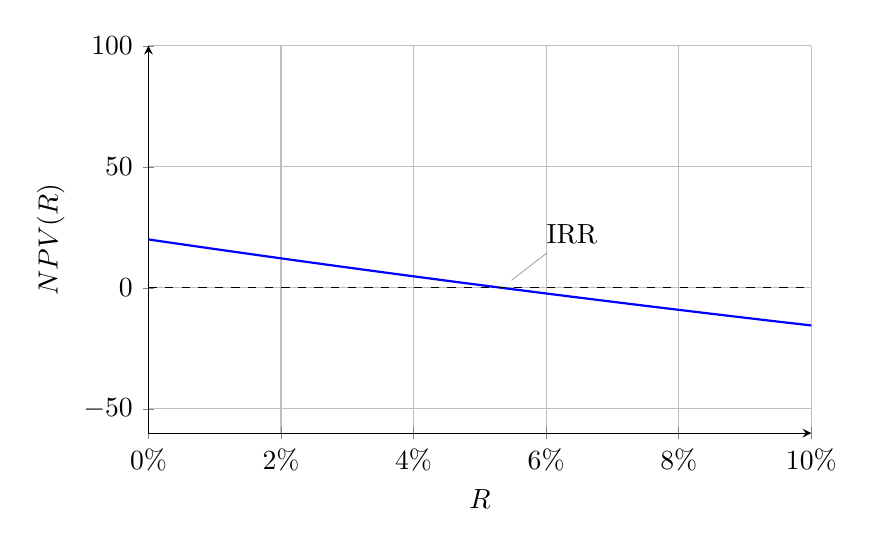
\begin{tikzpicture}
\begin{axis}[
  width=10cm, height=6.5cm,
  xlabel={$R$}, ylabel={$NPV(R)$},
  xmin=0, xmax=0.10, ymin=-60, ymax=100,
  xtick={0,0.02,0.04,0.06,0.08,0.10},
  xticklabel={\pgfmathparse{\tick*100}\pgfmathprintnumber{\pgfmathresult}\%},
  axis lines=left,
  grid=major]
\addplot[domain=0:0.10, samples=60, thick, blue]
  {200/(1+x) + 100/(1+x)^2 - 280};
\addplot[domain=0:0.10, samples=2, black, dashed] {0};
\node[pin=45:{IRR}] at (axis cs:0.0533,0) {};
\end{axis}
\end{tikzpicture}
\caption{NPV法とIRR法のイメージ。$NPV(R)$ は単調減少関数であり，横軸との交点が
IRR である。IRR と WACC の比較で投資判断を行う。}
\label{fig:npv-irr}
\end{figure}

\begin{example}[例題2-2]
以下の2種類の投資がある。
\begin{description}
\item[投資A.] 現時点で280億円の投資をすると，1年後に200億円，2年後に100億円の
キャッシュフローが確実に得られる。
\item[投資B.] 現時点で280億円の投資をすると，1年後に150億円，2年後に150億円の
キャッシュフローが確実に得られる。
\end{description}
(どちらも合計300億円が得られる設定である。)
\begin{enumerate}
\item[(1)] どちらに投資すべきか，IRR法を用いて判断しなさい。
\item[(2)] 割引率 $R = 4.5\%$ として，NPV法を用いて2種類の投資の妥当性について
述べなさい。
\end{enumerate}

\medskip
\noindent\textbf{解答。}
(1) 投資Aについて，IRR は
\[
\frac{200}{1+R} + \frac{100}{(1+R)^2} - 280 = 0
\]
の解であり，$R_A = 5.3342\%$。同様に投資Bでは
$\frac{150}{1+R} + \frac{150}{(1+R)^2} - 280 = 0$ の解として $R_B = 4.7255\%$ を
得る。IRR が高い投資Aを実行すべきである。

(2) 割引率 $R=4.5\%$ で計算すると，
\begin{align*}
NPV_A &= \frac{200}{1.045} + \frac{100}{1.045^2} - 280 = 2.960555\text{ 億円},\\
NPV_B &= \frac{150}{1.045} + \frac{150}{1.045^2} - 280 = 0.900163\text{ 億円}.
\end{align*}
どちらも $NPV>0$ なので，どちらの投資も合理的である。また，正味現在価値は
投資Aの方が高い。
\end{example}

\vspace{18pt}

\subsection{NPV法・IRR法で十分か?}

実際には，
\begin{itemize}
\item 将来キャッシュフローは不確実である場合が多い。
\item さらに，投資判断を行う時点は延期できることが多い。
\end{itemize}

将来キャッシュフローが不確実な場合の例を見てみよう。以下では一時的に，時間的な
価値の違い(時間による割引の効果)は無視して考える。

\begin{example}[将来キャッシュフローが不確実な場合]
「1年後に，50\%の確率で12億円，50\%の確率で8億円受け取れる」という投資のために
必要な金額が，現在は9億円であるとする。この投資の正味現在価値はいくらか。

正味現在価値の算出に期待値を使うならば，
\[
NPV = 0.5\times 12 + 0.5\times 8 - 9 = 1 > 0
\]
となる。しかし，この結果が $NPV>0$ だからといって，投資すべきと言えるだろうか。
この投資では，確率50\%で1億円の損失が発生する。この損失が投資家の経営に大きな
影響を与えうるとすれば，もう少し慎重に考えるべきではないだろうか。
\end{example}

この損失を重視する投資家は，何らかの(期待値とは別の)形で損失の効果を考慮した
投資評価を行う。\textbf{この評価の方法を提供するのが，金融工学}である。本講義の
後半で説明する。

\subsection*{参考：古いプロジェクト評価法}

参考までに，古いプロジェクト評価法を挙げる(講義では特に注意を払わなくて
よいとされた)。
\begin{itemize}
\item \textbf{回収期間法} (payback period method)：既に述べた。
\item \textbf{割引回収期間法} (discounted payback period method)：回収期間を，
回収額でなく，回収額の現在価値で求めたもの。
\item \textbf{収益性指標法} (profitability index method)：
(投資による将来CFの現在価値)/(初期投資額) $> 1$ ならば投資する。
\end{itemize}

% ---------------- 演習問題 ----------------
\section{演習問題}

\begin{exercise}[問題2-1]
複利利回り(年率)を5\%とする。
\begin{enumerate}
\item[(1)] いま100円投資したときの，3年後の価値(終価)。
\item[(2)] 3年後の100円の現在価値(現価)。
\end{enumerate}
これらを，(A) 1年複利，(B) 半年複利，(C) 3ヶ月複利，(D) 連続複利，のそれぞれの
場合について求めなさい。
\end{exercise}

\begin{answerbox}
\textbf{考え方。}例題2-1と同じ計算を，期間 $n=3$ 年に伸ばしたものである。
離散時間の一般形\eqref{eq:discrete-general}より，転化回数 $m$ のとき
\[
\text{終価} = 100\Bigl(1+\frac{0.05}{m}\Bigr)^{3m},
\qquad
\text{現価} = 100\Bigl(1+\frac{0.05}{m}\Bigr)^{-3m}
\]
であり，連続複利では式\eqref{eq:continuous-general}より終価 $100e^{0.05\times 3}$，
現価 $100e^{-0.05\times 3}$ となる。

\medskip
\textbf{計算。}
\begin{itemize}
\item[(A)] 1年複利($m=1$)：終価 $100\times 1.05^3 = 115.763$ 円，
現価 $100\times 1.05^{-3} = 86.384$ 円。
\item[(B)] 半年複利($m=2$)：終価 $100\times 1.025^6 = 115.969$ 円，
現価 $100\times 1.025^{-6} = 86.230$ 円。
\item[(C)] 3ヶ月複利($m=4$)：終価 $100\times 1.0125^{12} = 116.075$ 円，
現価 $100\times 1.0125^{-12} = 86.151$ 円。
\item[(D)] 連続複利：終価 $100e^{0.15} = 116.183$ 円，
現価 $100e^{-0.15} = 86.077$ 円。
\end{itemize}

\medskip
\textbf{ポイント。}同じ年率5\%でも，転化回数が多いほど再投資の効果が働いて終価は
大きくなり，その分だけ現価は小さくなる。連続複利が両者の極限(終価は上限，現価は
下限)を与える。
\end{answerbox}

\begin{exercise}[問題2-2]
例題2-2の設定のもとで，さらにもう一つの投資案件も考慮する。
\begin{description}
\item[投資C.] 現時点で280億円の投資をすると，1年後に100億円，2年後に200億円の
キャッシュフローが確実に得られる。
\end{description}
\begin{enumerate}
\item[(1)] どれに投資すべきか，IRR法を用いて判断しなさい。
\item[(2)] 割引率 $R = 4.5\%$ として，NPV法を用いて投資Cの妥当性について
述べなさい。
\end{enumerate}
\end{exercise}

\begin{answerbox}
\textbf{考え方。}投資Cは合計金額こそ投資A・Bと同じ300億円だが，大きい方の
キャッシュフロー(200億円)を受け取るのが2年後と遅い。時間価値を考えると，
同じ合計額でも受取が遅いほど価値は低いはずである。このことを IRR と NPV で
定量的に確認する。

\medskip
\textbf{(1) IRR法。}投資Cの IRR は
\[
\frac{100}{1+R} + \frac{200}{(1+R)^2} - 280 = 0
\]
の解である。これを解くと($x=1+R$ とおけば $280x^2 - 100x - 200 = 0$ という
2次方程式になる)$R_C = 4.2385\%$ を得る。3案件を並べると：
\vspace{0.9em}
\begin{center}
\begin{tabular}{lccc}
\toprule
時点 & 投資A & 投資B & 投資C\\
\midrule
0(投資額) & 280 & 280 & 280\\
1年後 & 200 & 150 & 100\\
2年後 & 100 & 150 & 200\\
\midrule
IRR & 5.3342\% & 4.7255\% & 4.2385\%\\
\bottomrule
\end{tabular}
\end{center}
\vspace{0.9em}
この結果より，IRR が最も高い\textbf{投資Aを実行すべき}である。

\medskip
\textbf{(2) NPV法。}割引率 $R=4.5\%$ として
\[
NPV_C = \frac{100}{1.045} + \frac{200}{1.045^2} - 280 = -1.16023\text{ 億円} < 0.
\]
\vspace{0.9em}
\begin{center}
\begin{tabular}{lccc}
\toprule
 & 投資A & 投資B & 投資C\\
\midrule
NPV(億円) & 2.960555 & 0.900163 & $-1.16023$\\
\bottomrule
\end{tabular}
\end{center}
\vspace{0.9em}
投資Cは正味現在価値がマイナスになるので，\textbf{非合理的な投資}と判断できる。

\medskip
\textbf{ポイント。}IRR と NPV の判定は整合的である。すなわち，
\[
\text{割引率} < IRR \;\to\; NPV > 0,
\qquad
\text{割引率} > IRR \;\to\; NPV < 0
\]
であり，NPV は $R$ の単調関数なので逆向きも成立する。実際，投資Cでは
IRR($4.2385\%$)$<$ 割引率($4.5\%$)なので $NPV<0$ となっている。また，
受取合計額が同じ300億円でも，早い時点に多く受け取る投資Aほど IRR・NPV ともに
高い。これはキャッシュフローの時間価値そのものである。
\end{answerbox}
